\documentclass{standalone}
\usepackage{color}
\usepackage{tikz}
\usepackage{animate}
\usepackage{calc}
\usepackage{mathabx}
\usetikzlibrary{arrows}
\usetikzlibrary{calc}
\usetikzlibrary{backgrounds}
\usetikzlibrary{shapes.arrows}

\begin{document}

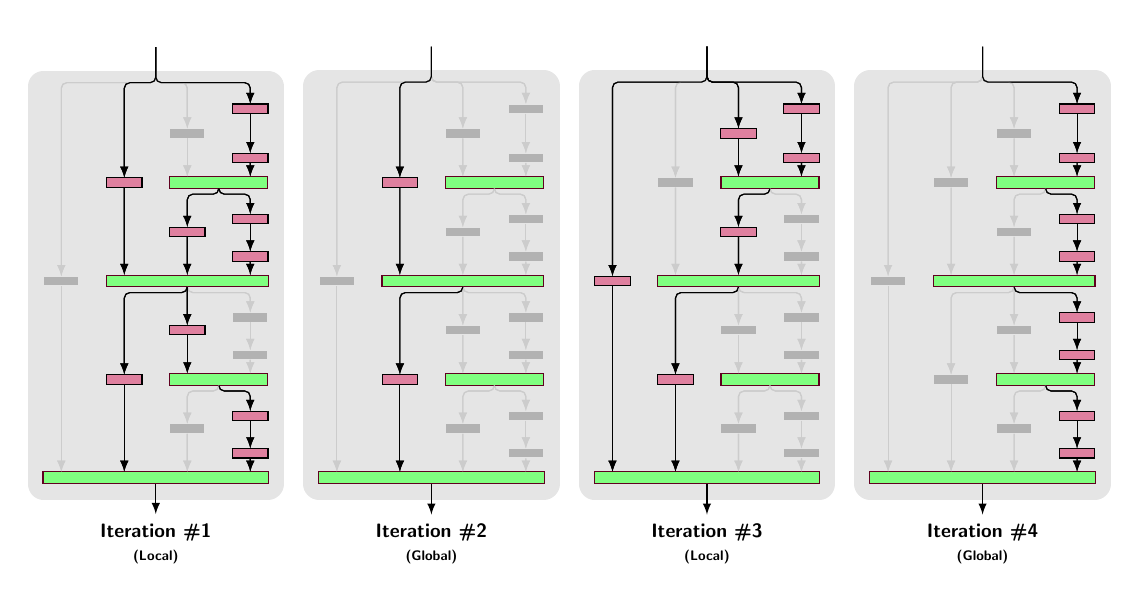
\begin{tikzpicture}[->,>=latex,auto,node distance=3cm,transform shape,
 thick,main node/.style={circle,draw,font=\sffamily\Large\bfseries}]
\def\blockheight{5.0}
\def\layerwidth{0.3}
\def\layerheight{0.04}
\def\columnwidth{0.8}
\def\iterwidth{3.5}
\def\one{0}
\def\two{\iterwidth}
\def\three{2*\iterwidth}
\def\four{3*\iterwidth}
\def\extrabufy{0.15}

\def\blocks{1}
\def\columns{4}

\def\arrowbuf{0.07}
\tikzstyle{noconv}=[rectangle,draw=black!10,thick,fill=black!30,thin,minimum width=1.5cm,minimum height=0.4cm,scale=0.3]
\tikzstyle{conv}=[rectangle,draw,thick,fill=purple!50,thin,minimum width=1.5cm,minimum height=0.4cm,scale=0.3]
\tikzstyle{pool}=[rectangle,draw,thick,fill=yellow!50,thin,minimum width=1.5cm,minimum height=0.4cm,scale=0.3]
\tikzstyle{dense}=[rectangle,draw,thick,fill=blue!50,thin,minimum width=1.5cm,minimum height=0.4cm,scale=0.3]
\tikzstyle{func}=[rectangle,draw,thick,fill=gray!50,thin,scale=1.0]
\tikzstyle{joiner}=[rectangle,thick,draw,fill=green!50,draw=black!50!purple,thin,minimum width=1.5cm,minimum height=0.5cm,scale=0.3]
\tikzstyle{joiner1}=[rectangle,thick,draw,fill=green!50,draw=black!50!purple,thin,minimum width=9.55cm,minimum height=0.5cm,scale=0.3]
\tikzstyle{joiner2}=[rectangle,thick,draw,fill=green!50,draw=black!50!purple,thin,minimum width=6.85cm,minimum height=0.5cm,scale=0.3]
\tikzstyle{joiner3}=[rectangle,thick,draw,fill=green!50,draw=black!50!purple,thin,minimum width=4.15cm,minimum height=0.5cm,scale=0.3]
\tikzstyle{myround}=[rounded corners=0.07cm]
\tikzstyle{arrow}=[->,thin]
\tikzstyle{noarrow}=[->,thin,black!20]

\foreach \b in {1, \blocks} {
    \node[joiner1] (joiner-\b-1-1) at (\one+\columnwidth*\columns/2, -\b*\blockheight) {};
    \foreach \j in {1, ..., 1} {
        \node[joiner2] (joiner-\b-2-\j) at (\one+\columnwidth*2.5, -\b*\blockheight +\blockheight -\blockheight/2 - \j*\blockheight/1 + \blockheight/1) {};
    }
    \foreach \j in {1, ..., 2} {
        \node[joiner3] (joiner-\b-3-\j) at (\one+\columnwidth*3, -\b*\blockheight +\blockheight -\blockheight/4 - \j*\blockheight/2 + \blockheight/2) {};
    }
    \foreach \c/\layers in {1/1, 2/2, 3/4, 4/8} {
        \def\x{\one+\c*\columnwidth - \columnwidth/2}
        \def\y{\blockheight-\b*\blockheight}
        \def\convradius{\blockheight/\layers}
        \foreach \n in {1, ..., \layers} {
            \ifthenelse{\c=4 \AND \n=3}{
                \def\yn{\y - \n*\convradius + 0.5*\convradius - \extrabufy}
            }{
                \ifthenelse{\c=4 \AND \n=5}{
                    \def\yn{\y - \n*\convradius + 0.5*\convradius - \extrabufy}
                }{
                    \ifthenelse{\c=4 \AND \n=7}{
                        \def\yn{\y - \n*\convradius + 0.5*\convradius - \extrabufy}
                    }{
                        \def\yn{\y - \n*\convradius + 0.5*\convradius}
                    }
                }
            }
            \def\xn{\x}
            % ugly fix: and/or not working as expected
            \ifthenelse{\c=1 \AND \n=1 \OR \c=3 \AND \n=1}{
                \node[noconv] (conv-\b-\c-\n) at (\xn, \yn) {};
            }{
                \ifthenelse{\c=4 \AND \n=5}{
                    \node[noconv] (conv-\b-\c-\n) at (\xn, \yn) {};
                }{
                    \ifthenelse{\c=4 \AND \n=6}{
                        \node[noconv] (conv-\b-\c-\n) at (\xn, \yn) {};
                    }{
                        \ifthenelse{\c=3 \AND \n=4}{
                            \node[noconv] (conv-\b-\c-\n) at (\xn, \yn) {};
                        }{
                            \node[conv] (conv-\b-\c-\n) at (\xn, \yn) {};
                        }
                    }
                }
            }
        }
    }

    \node (entry) at (\one+\columnwidth*\columns/2, 0.6) {};
    \node (below-entry) at (\one+\columnwidth*\columns/2, 0.1) {};

    \draw[noarrow,myround] (entry.south) to ($(entry.south) + (0, -0.45)$) to ($(entry.south) + (+\columnwidth*0.5, -0.45)$) to  (conv-\b-3-1);
    \draw[noarrow,myround] (entry.south) to ($(entry.south) + (0, -0.45)$) to ($(entry.south) + (-\columnwidth*1.5, -0.45)$) to  (conv-\b-1-1);
    \draw[arrow,myround] (entry.south) to ($(entry.south) + (0, -0.45)$) to ($(entry.south) + (+\columnwidth*1.5, -0.45)$) to  (conv-\b-4-1);
    \draw[arrow,myround] (entry.south) to ($(entry.south) + (0, -0.45)$) to ($(entry.south) + (-\columnwidth*0.5, -0.45)$) to  (conv-\b-2-1);

    \draw[noarrow,myround] (joiner-\b-2-1.south) to ($(joiner-\b-2-1.south) + (0, -\arrowbuf)$) to ($(joiner-\b-2-1.south) + (\columnwidth, -\arrowbuf)$) to (conv-\b-4-5);
    \draw[noarrow] (conv-\b-4-5) to (conv-\b-4-6);
    \draw[noarrow] (conv-\b-4-6) to ($(joiner-\b-3-2.north) + (\columnwidth/2, 0)$);
    \draw[noarrow,myround] (joiner-\b-3-2.south) to ($(joiner-\b-3-2.south) + (0, -\arrowbuf)$) to ($(joiner-\b-3-2.south) + (-\columnwidth/2, -\arrowbuf)$) to (conv-\b-3-4);
    \draw[noarrow] (conv-\b-3-4) to ($(joiner-\b-1-1.north) + (\columnwidth*0.5, 0)$);
    \draw[noarrow] (conv-\b-1-1) to ($(joiner-\b-1-1.north) - (\columnwidth*1.5, 0)$);
    \draw[arrow] (conv-\b-4-1) to (conv-\b-4-2);
    \draw[arrow] (conv-\b-4-2) to ($(joiner-\b-3-1.north) + (\columnwidth/2, 0)$);
    %\draw[arrow] ($(joiner-\b-3-1.south) + (\columnwidth/2, 0)$) to (conv-\b-4-3);
    \draw[arrow,myround] (joiner-\b-3-1.south) to ($(joiner-\b-3-1.south) + (0, -\arrowbuf)$) to ($(joiner-\b-3-1.south) + (\columnwidth/2, -\arrowbuf)$) to (conv-\b-4-3);
    \draw[arrow] (conv-\b-4-3) to (conv-\b-4-4);
    \draw[arrow] (conv-\b-4-4) to ($(joiner-\b-2-1.north) + (\columnwidth, 0)$);
    %\draw[arrow] ($(joiner-\b-2-1.south) + (\columnwidth, 0)$) to (conv-\b-4-5);
    %\draw[arrow] ($(joiner-\b-3-2.south) + (\columnwidth/2, 0)$) to (conv-\b-4-7);
    \draw[arrow,myround] (joiner-\b-3-2.south) to ($(joiner-\b-3-2.south) + (0, -\arrowbuf)$) to ($(joiner-\b-3-2.south) + (\columnwidth/2, -\arrowbuf)$) to (conv-\b-4-7);
    \draw[arrow] (conv-\b-4-7) to (conv-\b-4-8);
    \draw[arrow] (conv-\b-4-8) to ($(joiner-\b-1-1.north) + (\columnwidth*1.5, 0)$);


    \draw[noarrow] (conv-\b-3-1) to ($(joiner-\b-3-1.north) - (\columnwidth/2, 0)$);
    %\draw[arrow] ($(joiner-\b-3-1.south) - (\columnwidth/2, 0)$) to (conv-\b-3-2);
    \draw[arrow,myround] (joiner-\b-3-1.south) to ($(joiner-\b-3-1.south) + (0, -\arrowbuf)$)  to ($(joiner-\b-3-1.south) + (-\columnwidth/2, -\arrowbuf)$)  to (conv-\b-3-2);
    \draw[arrow] (conv-\b-3-2) to (joiner-\b-2-1);
    \draw[arrow] (joiner-\b-2-1) to (conv-\b-3-3);
    \draw[arrow] (conv-\b-3-3) to ($(joiner-\b-3-2.north) - (\columnwidth/2, 0)$);
    %\draw[arrow] ($(joiner-\b-3-2.south) - (\columnwidth/2, 0)$) to (conv-\b-3-4);

    \draw[arrow] (conv-\b-2-1) to ($(joiner-\b-2-1.north) - (\columnwidth, 0)$);
    %\draw[arrow] ($(joiner-\b-2-1.south) - (\columnwidth, 0)$) to (conv-\b-2-2);
    \draw[arrow,myround] (joiner-\b-2-1.south) to ($(joiner-\b-2-1.south) + (0, -\arrowbuf)$) to ($(joiner-\b-2-1.south) + (-\columnwidth, -\arrowbuf)$) to (conv-\b-2-2);
    \draw[arrow] (conv-\b-2-2) to ($(joiner-\b-1-1.north) + (-\columnwidth*0.5, 0)$);


}

\node (exit) at (\one+\columnwidth*\columns/2, -\blocks*\blockheight-0.7) {\textbf{\textsf{\scriptsize{Iteration \#1}}}};
\node (exit-south) at (\one+\columnwidth*\columns/2, -\blocks*\blockheight-1.0) {\textbf{\textsf{\tiny{(Local)}}}};
%\draw[arrow] (joiner-2-1-1) to  (exit);
\draw[arrow] (joiner-1-1-1) to  (exit);

\begin{pgfonlayer}{background}
\filldraw [line width=4mm,join=round,black!10]
  (below-entry.south -| conv-1-4-1.east) rectangle (joiner-1-1-1.south -| conv-1-1-1.west);
\end{pgfonlayer}

\foreach \b in {1, \blocks} {
    \node[joiner1] (joiner-\b-1-1) at (\two+\columnwidth*\columns/2, -\b*\blockheight) {};
    \foreach \j in {1, ..., 1} {
        \node[joiner2] (joiner-\b-2-\j) at (\two+\columnwidth*2.5, -\b*\blockheight +\blockheight -\blockheight/2 - \j*\blockheight/1 + \blockheight/1) {};
    }
    \foreach \j in {1, ..., 2} {
        \node[joiner3] (joiner-\b-3-\j) at (\two+\columnwidth*3, -\b*\blockheight +\blockheight -\blockheight/4 - \j*\blockheight/2 + \blockheight/2) {};
    }
    \foreach \c/\layers in {1/1, 2/2, 3/4, 4/8} {
        \def\x{\two+\c*\columnwidth - \columnwidth/2}
        \def\y{\blockheight-\b*\blockheight}
        \def\convradius{\blockheight/\layers}
        \foreach \n in {1, ..., \layers} {
            \ifthenelse{\c=4 \AND \n=3}{
                \def\yn{\y - \n*\convradius + 0.5*\convradius - \extrabufy}
            }{
                \ifthenelse{\c=4 \AND \n=5}{
                    \def\yn{\y - \n*\convradius + 0.5*\convradius - \extrabufy}
                }{
                    \ifthenelse{\c=4 \AND \n=7}{
                        \def\yn{\y - \n*\convradius + 0.5*\convradius - \extrabufy}
                    }{
                        \def\yn{\y - \n*\convradius + 0.5*\convradius}
                    }
                }
            }
            \def\xn{\x}
            \ifthenelse{\c=2}{
                \node[conv] (conv-\b-\c-\n) at (\xn, \yn) {};
            }{
                \node[noconv] (conv-\b-\c-\n) at (\xn, \yn) {};
            }
        }
    }

    \node (entry) at (\two+\columnwidth*\columns/2, 0.6) {};
    \node (below-entry) at (\two+\columnwidth*\columns/2, 0.1) {};

    \draw[noarrow,myround] (entry.south) to ($(entry.south) + (0, -0.45)$) to ($(entry.south) + (+\columnwidth*0.5, -0.45)$) to  (conv-\b-3-1);
    \draw[noarrow,myround] (entry.south) to ($(entry.south) + (0, -0.45)$) to ($(entry.south) + (-\columnwidth*1.5, -0.45)$) to  (conv-\b-1-1);
    \draw[noarrow,myround] (entry.south) to ($(entry.south) + (0, -0.45)$) to ($(entry.south) + (+\columnwidth*1.5, -0.45)$) to  (conv-\b-4-1);
    \draw[arrow,myround] (entry.south) to ($(entry.south) + (0, -0.45)$) to ($(entry.south) + (-\columnwidth*0.5, -0.45)$) to  (conv-\b-2-1);

    \draw[noarrow] (conv-\b-4-1) to (conv-\b-4-2);
    \draw[noarrow] (conv-\b-4-2) to ($(joiner-\b-3-1.north) + (\columnwidth/2, 0)$);
    %\draw[arrow] ($(joiner-\b-3-1.south) + (\columnwidth/2, 0)$) to (conv-\b-4-3);
    \draw[noarrow,myround] (joiner-\b-3-1.south) to ($(joiner-\b-3-1.south) + (0, -\arrowbuf)$) to ($(joiner-\b-3-1.south) + (\columnwidth/2, -\arrowbuf)$) to (conv-\b-4-3);
    \draw[noarrow] (conv-\b-4-3) to (conv-\b-4-4);
    \draw[noarrow] (conv-\b-4-4) to ($(joiner-\b-2-1.north) + (\columnwidth, 0)$);
    %\draw[arrow] ($(joiner-\b-2-1.south) + (\columnwidth, 0)$) to (conv-\b-4-5);
    \draw[noarrow,myround] (joiner-\b-2-1.south) to ($(joiner-\b-2-1.south) + (0, -\arrowbuf)$) to ($(joiner-\b-2-1.south) + (\columnwidth, -\arrowbuf)$) to (conv-\b-4-5);
    \draw[noarrow] (conv-\b-4-5) to (conv-\b-4-6);
    \draw[noarrow] (conv-\b-4-6) to ($(joiner-\b-3-2.north) + (\columnwidth/2, 0)$);
    %\draw[arrow] ($(joiner-\b-3-2.south) + (\columnwidth/2, 0)$) to (conv-\b-4-7);
    \draw[noarrow,myround] (joiner-\b-3-2.south) to ($(joiner-\b-3-2.south) + (0, -\arrowbuf)$) to ($(joiner-\b-3-2.south) + (\columnwidth/2, -\arrowbuf)$) to (conv-\b-4-7);
    \draw[noarrow] (conv-\b-4-7) to (conv-\b-4-8);
    \draw[noarrow] (conv-\b-4-8) to ($(joiner-\b-1-1.north) + (\columnwidth*1.5, 0)$);


    \draw[noarrow] (conv-\b-3-1) to ($(joiner-\b-3-1.north) - (\columnwidth/2, 0)$);
    %\draw[arrow] ($(joiner-\b-3-1.south) - (\columnwidth/2, 0)$) to (conv-\b-3-2);
    \draw[noarrow,myround] (joiner-\b-3-1.south) to ($(joiner-\b-3-1.south) + (0, -\arrowbuf)$)  to ($(joiner-\b-3-1.south) + (-\columnwidth/2, -\arrowbuf)$)  to (conv-\b-3-2);
    \draw[noarrow] (conv-\b-3-2) to (joiner-\b-2-1);
    \draw[noarrow] (joiner-\b-2-1) to (conv-\b-3-3);
    \draw[noarrow] (conv-\b-3-3) to ($(joiner-\b-3-2.north) - (\columnwidth/2, 0)$);
    %\draw[arrow] ($(joiner-\b-3-2.south) - (\columnwidth/2, 0)$) to (conv-\b-3-4);
    \draw[noarrow,myround] (joiner-\b-3-2.south) to ($(joiner-\b-3-2.south) + (0, -\arrowbuf)$) to ($(joiner-\b-3-2.south) + (-\columnwidth/2, -\arrowbuf)$) to (conv-\b-3-4);
    \draw[noarrow] (conv-\b-3-4) to ($(joiner-\b-1-1.north) + (\columnwidth*0.5, 0)$);

    \draw[noarrow] (conv-\b-1-1) to ($(joiner-\b-1-1.north) - (\columnwidth*1.5, 0)$);

    \draw[arrow] (conv-\b-2-1) to ($(joiner-\b-2-1.north) - (\columnwidth, 0)$);
    %\draw[arrow] ($(joiner-\b-2-1.south) - (\columnwidth, 0)$) to (conv-\b-2-2);
    \draw[arrow,myround] (joiner-\b-2-1.south) to ($(joiner-\b-2-1.south) + (0, -\arrowbuf)$) to ($(joiner-\b-2-1.south) + (-\columnwidth, -\arrowbuf)$) to (conv-\b-2-2);
    \draw[arrow] (conv-\b-2-2) to ($(joiner-\b-1-1.north) + (-\columnwidth*0.5, 0)$);


}

\node (exit) at (\two+\columnwidth*\columns/2, -\blocks*\blockheight-0.7) {\textbf{\textsf{\scriptsize{Iteration \#2}}}};
\node (exit-south) at (\two+\columnwidth*\columns/2, -\blocks*\blockheight-1.0) {\textbf{\textsf{\tiny{(Global)}}}};
%\draw[arrow] (joiner-2-1-1) to  (exit);
\draw[arrow] (joiner-1-1-1) to  (exit);

\begin{pgfonlayer}{background}
\filldraw [line width=4mm,join=round,black!10]
  (below-entry.south -| conv-1-4-1.east) rectangle (joiner-1-1-1.south -| conv-1-1-1.west);
\end{pgfonlayer}

\foreach \b in {1, \blocks} {
    \node[joiner1] (joiner-\b-1-1) at (\three+\columnwidth*\columns/2, -\b*\blockheight) {};
    \foreach \j in {1, ..., 1} {
        \node[joiner2] (joiner-\b-2-\j) at (\three+\columnwidth*2.5, -\b*\blockheight +\blockheight -\blockheight/2 - \j*\blockheight/1 + \blockheight/1) {};
    }
    \foreach \j in {1, ..., 2} {
        \node[joiner3] (joiner-\b-3-\j) at (\three+\columnwidth*3, -\b*\blockheight +\blockheight -\blockheight/4 - \j*\blockheight/2 + \blockheight/2) {};
    }
    \foreach \c/\layers in {1/1, 2/2, 3/4, 4/8} {
        \def\x{\three+\c*\columnwidth - \columnwidth/2}
        \def\y{\blockheight-\b*\blockheight}
        \def\convradius{\blockheight/\layers}
        \foreach \n in {1, ..., \layers} {
            \ifthenelse{\c=4 \AND \n=3}{
                \def\yn{\y - \n*\convradius + 0.5*\convradius - \extrabufy}
            }{
                \ifthenelse{\c=4 \AND \n=5}{
                    \def\yn{\y - \n*\convradius + 0.5*\convradius - \extrabufy}
                }{
                    \ifthenelse{\c=4 \AND \n=7}{
                        \def\yn{\y - \n*\convradius + 0.5*\convradius - \extrabufy}
                    }{
                        \def\yn{\y - \n*\convradius + 0.5*\convradius}
                    }
                }
            }
            \def\xn{\x}
            \ifthenelse{\c=2 \AND \n=1}{
                \node[noconv] (conv-\b-\c-\n) at (\xn, \yn) {};
            }{
                \ifthenelse{\c=3 \AND \n=3}{
                    \node[noconv] (conv-\b-\c-\n) at (\xn, \yn) {};
                }{
                    \ifthenelse{\c=3 \AND \n=4}{
                        \node[noconv] (conv-\b-\c-\n) at (\xn, \yn) {};
                    }{

                        \ifthenelse{\c=4}{
                            \ifthenelse{\n=1 \OR \n=2}{
                                \node[conv] (conv-\b-\c-\n) at (\xn, \yn) {};
                            }{
                                \node[noconv] (conv-\b-\c-\n) at (\xn, \yn) {};
                            }
                        }{
                            \node[conv] (conv-\b-\c-\n) at (\xn, \yn) {};
                        }
                    }
                }
            }
        }
    }

    \node (entry) at (\three+\columnwidth*\columns/2, 0.6) {};
    \node (below-entry) at (\three+\columnwidth*\columns/2, 0.1) {};

    \draw[noarrow,myround] (entry.south) to ($(entry.south) + (0, -0.45)$) to ($(entry.south) + (-\columnwidth*0.5, -0.45)$) to  (conv-\b-2-1);
    \draw[arrow,myround] (entry.south) to ($(entry.south) + (0, -0.45)$) to ($(entry.south) + (+\columnwidth*0.5, -0.45)$) to  (conv-\b-3-1);
    \draw[arrow,myround] (entry.south) to ($(entry.south) + (0, -0.45)$) to ($(entry.south) + (-\columnwidth*1.5, -0.45)$) to  (conv-\b-1-1);
    \draw[arrow,myround] (entry.south) to ($(entry.south) + (0, -0.45)$) to ($(entry.south) + (+\columnwidth*1.5, -0.45)$) to  (conv-\b-4-1);

    \draw[arrow] (conv-\b-4-1) to (conv-\b-4-2);
    \draw[arrow] (conv-\b-4-2) to ($(joiner-\b-3-1.north) + (\columnwidth/2, 0)$);
    %\draw[arrow] ($(joiner-\b-3-1.south) + (\columnwidth/2, 0)$) to (conv-\b-4-3);
    \draw[noarrow,myround] (joiner-\b-3-1.south) to ($(joiner-\b-3-1.south) + (0, -\arrowbuf)$) to ($(joiner-\b-3-1.south) + (\columnwidth/2, -\arrowbuf)$) to (conv-\b-4-3);
    \draw[noarrow] (conv-\b-4-3) to (conv-\b-4-4);
    \draw[noarrow] (conv-\b-4-4) to ($(joiner-\b-2-1.north) + (\columnwidth, 0)$);
    %\draw[arrow] ($(joiner-\b-2-1.south) + (\columnwidth, 0)$) to (conv-\b-4-5);
    \draw[noarrow,myround] (joiner-\b-2-1.south) to ($(joiner-\b-2-1.south) + (0, -\arrowbuf)$) to ($(joiner-\b-2-1.south) + (\columnwidth, -\arrowbuf)$) to (conv-\b-4-5);
    \draw[noarrow] (conv-\b-4-5) to (conv-\b-4-6);
    \draw[noarrow] (conv-\b-4-6) to ($(joiner-\b-3-2.north) + (\columnwidth/2, 0)$);
    %\draw[arrow] ($(joiner-\b-3-2.south) + (\columnwidth/2, 0)$) to (conv-\b-4-7);
    \draw[noarrow,myround] (joiner-\b-3-2.south) to ($(joiner-\b-3-2.south) + (0, -\arrowbuf)$) to ($(joiner-\b-3-2.south) + (\columnwidth/2, -\arrowbuf)$) to (conv-\b-4-7);
    \draw[noarrow] (conv-\b-4-7) to (conv-\b-4-8);
    \draw[noarrow] (conv-\b-4-8) to ($(joiner-\b-1-1.north) + (\columnwidth*1.5, 0)$);


    \draw[noarrow] (joiner-\b-2-1) to (conv-\b-3-3);
    \draw[noarrow] (conv-\b-3-3) to ($(joiner-\b-3-2.north) - (\columnwidth/2, 0)$);
    %\draw[arrow] ($(joiner-\b-3-2.south) - (\columnwidth/2, 0)$) to (conv-\b-3-4);
    \draw[noarrow,myround] (joiner-\b-3-2.south) to ($(joiner-\b-3-2.south) + (0, -\arrowbuf)$) to ($(joiner-\b-3-2.south) + (-\columnwidth/2, -\arrowbuf)$) to (conv-\b-3-4);
    \draw[noarrow] (conv-\b-3-4) to ($(joiner-\b-1-1.north) + (\columnwidth*0.5, 0)$);

    \draw[noarrow] (conv-\b-2-1) to ($(joiner-\b-2-1.north) - (\columnwidth, 0)$);
    %\draw[arrow] ($(joiner-\b-2-1.south) - (\columnwidth, 0)$) to (conv-\b-2-2);

    \draw[arrow] (conv-\b-3-1) to ($(joiner-\b-3-1.north) - (\columnwidth/2, 0)$);
    %\draw[arrow] ($(joiner-\b-3-1.south) - (\columnwidth/2, 0)$) to (conv-\b-3-2);
    \draw[arrow,myround] (joiner-\b-3-1.south) to ($(joiner-\b-3-1.south) + (0, -\arrowbuf)$)  to ($(joiner-\b-3-1.south) + (-\columnwidth/2, -\arrowbuf)$)  to (conv-\b-3-2);
    \draw[arrow] (conv-\b-3-2) to (joiner-\b-2-1);
    \draw[arrow,myround] (joiner-\b-2-1.south) to ($(joiner-\b-2-1.south) + (0, -\arrowbuf)$) to ($(joiner-\b-2-1.south) + (-\columnwidth, -\arrowbuf)$) to (conv-\b-2-2);
    \draw[arrow] (conv-\b-2-2) to ($(joiner-\b-1-1.north) + (-\columnwidth*0.5, 0)$);

    \draw[arrow] (conv-\b-1-1) to ($(joiner-\b-1-1.north) - (\columnwidth*1.5, 0)$);

}

\node (exit) at (\three+\columnwidth*\columns/2, -\blocks*\blockheight-0.7) {\textbf{\textsf{\scriptsize{Iteration \#3}}}};
\node (exit-south) at (\three+\columnwidth*\columns/2, -\blocks*\blockheight-1.0) {\textbf{\textsf{\tiny{(Local)}}}};
%\draw[arrow] (joiner-2-1-1) to  (exit);
\draw[arrow] (joiner-1-1-1) to  (exit);

\begin{pgfonlayer}{background}
\filldraw [line width=4mm,join=round,black!10]
  (below-entry.south -| conv-1-4-1.east) rectangle (joiner-1-1-1.south -| conv-1-1-1.west);
\end{pgfonlayer}

\foreach \b in {1, \blocks} {
    \node[joiner1] (joiner-\b-1-1) at (\four+\columnwidth*\columns/2, -\b*\blockheight) {};
    \foreach \j in {1, ..., 1} {
        \node[joiner2] (joiner-\b-2-\j) at (\four+\columnwidth*2.5, -\b*\blockheight +\blockheight -\blockheight/2 - \j*\blockheight/1 + \blockheight/1) {};
    }
    \foreach \j in {1, ..., 2} {
        \node[joiner3] (joiner-\b-3-\j) at (\four+\columnwidth*3, -\b*\blockheight +\blockheight -\blockheight/4 - \j*\blockheight/2 + \blockheight/2) {};
    }
    \foreach \c/\layers in {1/1, 2/2, 3/4, 4/8} {
        \def\x{\four+\c*\columnwidth - \columnwidth/2}
        \def\y{\blockheight-\b*\blockheight}
        \def\convradius{\blockheight/\layers}
        \foreach \n in {1, ..., \layers} {
            \ifthenelse{\c=4 \AND \n=3}{
                \def\yn{\y - \n*\convradius + 0.5*\convradius - \extrabufy}
            }{
                \ifthenelse{\c=4 \AND \n=5}{
                    \def\yn{\y - \n*\convradius + 0.5*\convradius - \extrabufy}
                }{
                    \ifthenelse{\c=4 \AND \n=7}{
                        \def\yn{\y - \n*\convradius + 0.5*\convradius - \extrabufy}
                    }{
                        \def\yn{\y - \n*\convradius + 0.5*\convradius}
                    }
                }
            }
            \def\xn{\x}
            \ifthenelse{\c=4}{
                \node[conv] (conv-\b-\c-\n) at (\xn, \yn) {};
            }{
                \node[noconv] (conv-\b-\c-\n) at (\xn, \yn) {};
            }
        }
    }

    \node (entry) at (\four+\columnwidth*\columns/2, 0.6) {};
    \node (below-entry) at (\four+\columnwidth*\columns/2, 0.1) {};

    \draw[noarrow,myround] (entry.south) to ($(entry.south) + (0, -0.45)$) to ($(entry.south) + (+\columnwidth*0.5, -0.45)$) to  (conv-\b-3-1);
    \draw[noarrow,myround] (entry.south) to ($(entry.south) + (0, -0.45)$) to ($(entry.south) + (-\columnwidth*1.5, -0.45)$) to  (conv-\b-1-1);
    \draw[noarrow,myround] (entry.south) to ($(entry.south) + (0, -0.45)$) to ($(entry.south) + (-\columnwidth*0.5, -0.45)$) to  (conv-\b-2-1);
    \draw[arrow,myround] (entry.south) to ($(entry.south) + (0, -0.45)$) to ($(entry.south) + (+\columnwidth*1.5, -0.45)$) to  (conv-\b-4-1);


    \draw[noarrow] (conv-\b-3-1) to ($(joiner-\b-3-1.north) - (\columnwidth/2, 0)$);
    %\draw[arrow] ($(joiner-\b-3-1.south) - (\columnwidth/2, 0)$) to (conv-\b-3-2);
    \draw[noarrow,myround] (joiner-\b-3-1.south) to ($(joiner-\b-3-1.south) + (0, -\arrowbuf)$)  to ($(joiner-\b-3-1.south) + (-\columnwidth/2, -\arrowbuf)$)  to (conv-\b-3-2);
    \draw[noarrow] (conv-\b-3-2) to (joiner-\b-2-1);
    \draw[noarrow] (joiner-\b-2-1) to (conv-\b-3-3);
    \draw[noarrow] (conv-\b-3-3) to ($(joiner-\b-3-2.north) - (\columnwidth/2, 0)$);
    %\draw[arrow] ($(joiner-\b-3-2.south) - (\columnwidth/2, 0)$) to (conv-\b-3-4);
    \draw[noarrow,myround] (joiner-\b-3-2.south) to ($(joiner-\b-3-2.south) + (0, -\arrowbuf)$) to ($(joiner-\b-3-2.south) + (-\columnwidth/2, -\arrowbuf)$) to (conv-\b-3-4);
    \draw[noarrow] (conv-\b-3-4) to ($(joiner-\b-1-1.north) + (\columnwidth*0.5, 0)$);

    \draw[noarrow] (conv-\b-2-1) to ($(joiner-\b-2-1.north) - (\columnwidth, 0)$);
    %\draw[arrow] ($(joiner-\b-2-1.south) - (\columnwidth, 0)$) to (conv-\b-2-2);
    \draw[noarrow,myround] (joiner-\b-2-1.south) to ($(joiner-\b-2-1.south) + (0, -\arrowbuf)$) to ($(joiner-\b-2-1.south) + (-\columnwidth, -\arrowbuf)$) to (conv-\b-2-2);
    \draw[noarrow] (conv-\b-2-2) to ($(joiner-\b-1-1.north) + (-\columnwidth*0.5, 0)$);

    \draw[noarrow] (conv-\b-1-1) to ($(joiner-\b-1-1.north) - (\columnwidth*1.5, 0)$);

    \draw[arrow] (conv-\b-4-1) to (conv-\b-4-2);
    \draw[arrow] (conv-\b-4-2) to ($(joiner-\b-3-1.north) + (\columnwidth/2, 0)$);
    %\draw[arrow] ($(joiner-\b-3-1.south) + (\columnwidth/2, 0)$) to (conv-\b-4-3);
    \draw[arrow,myround] (joiner-\b-3-1.south) to ($(joiner-\b-3-1.south) + (0, -\arrowbuf)$) to ($(joiner-\b-3-1.south) + (\columnwidth/2, -\arrowbuf)$) to (conv-\b-4-3);
    \draw[arrow] (conv-\b-4-3) to (conv-\b-4-4);
    \draw[arrow] (conv-\b-4-4) to ($(joiner-\b-2-1.north) + (\columnwidth, 0)$);
    %\draw[arrow] ($(joiner-\b-2-1.south) + (\columnwidth, 0)$) to (conv-\b-4-5);
    \draw[arrow,myround] (joiner-\b-2-1.south) to ($(joiner-\b-2-1.south) + (0, -\arrowbuf)$) to ($(joiner-\b-2-1.south) + (\columnwidth, -\arrowbuf)$) to (conv-\b-4-5);
    \draw[arrow] (conv-\b-4-5) to (conv-\b-4-6);
    \draw[arrow] (conv-\b-4-6) to ($(joiner-\b-3-2.north) + (\columnwidth/2, 0)$);
    %\draw[arrow] ($(joiner-\b-3-2.south) + (\columnwidth/2, 0)$) to (conv-\b-4-7);
    \draw[arrow,myround] (joiner-\b-3-2.south) to ($(joiner-\b-3-2.south) + (0, -\arrowbuf)$) to ($(joiner-\b-3-2.south) + (\columnwidth/2, -\arrowbuf)$) to (conv-\b-4-7);
    \draw[arrow] (conv-\b-4-7) to (conv-\b-4-8);
    \draw[arrow] (conv-\b-4-8) to ($(joiner-\b-1-1.north) + (\columnwidth*1.5, 0)$);


}

\node (exit) at (\four+\columnwidth*\columns/2, -\blocks*\blockheight-0.7) {\textbf{\textsf{\scriptsize{Iteration \#4}}}};
\node (exit-south) at (\four+\columnwidth*\columns/2, -\blocks*\blockheight-1.0) {\textbf{\textsf{\tiny{(Global)}}}};
%\draw[arrow] (joiner-2-1-1) to  (exit);
\draw[arrow] (joiner-1-1-1) to  (exit);

\begin{pgfonlayer}{background}
\filldraw [line width=4mm,join=round,black!10]
  (below-entry.south -| conv-1-4-1.east) rectangle (joiner-1-1-1.south -| conv-1-1-1.west);
\end{pgfonlayer}

\end{tikzpicture}

\end{document}
